\chapter{Implementacja metod akceleracji i~rezultaty pomiarów}
\label{sec:methods-results}

W rozdziale tym opisane zostały sposoby implementacji badanych metod akceleracji obliczeń oraz zaprezentowany zostały rezultaty przeprowadzonych testów wydajności. Wskazane zostały również na wszelkie aspekty, na które trzeba zwrócić uwagę w~procesie budowania bibliotek z~daną metodę akceleracji oraz ich możliwości i~ograniczenia. Wszystkie wyniki pomiarów porównane zostały do wykonania sekwencyjnego w~C++, a~dla pozostałych metod akceleracji na wykresach kolorem szarym zaznaczony został zakres czasów wykonania sekwencyjnego wszystkich środowisk języka JavaScript.

Jak już wcześniej wspomniano w~rozdziale \ref{sec:benchmark}, dla każdej z~metod akceleracji zaimplementowano trzy algorytmy. Niżej przedstawiono nazwy i~oznaczenia używane na potrzeby implementacji i~prezentacji wyników.

\begin{itemize}
    \item Standard Hough Transform (SHT \textit{non-LUT}, \lstinline{SHT_Simple}) -- algorytm detekcji linii wykorzystujący intensywne obliczenia z~użyciem funkcji trygonometrycznych.
    \item Standard Hough Transform (SHT \textit{LUT}, \lstinline{SHT_Simple_Lookup}) -- algorytm detekcji linii wykorzystujący tablicę LUT do zapisanie potrzebnych wartości funkcji trygonometrycznych.
    \item Circle Hough Transform (CHT, \lstinline{CHT_Simple}) -- algorytm detekcji okręgów wykorzystujący metodę gradientu w~celu redukcji złożoności obliczeniowej (rozmiaru akumulatora). Zmienny parametr maksymalnego promienia obliczany jest ze wzoru $r_{max} = 20+10n$, gdzie $n$ to współczynnik inkrementowany w~kolejnych iteracjach pomiarów.
\end{itemize}


\section{Wykonanie sekwencyjne}

Implementacja procesu budowania biblioteki z~algorytmem transformacji w~wariancie wykonania sekwencyjnego nie wymagała zmian w~procesie budowania w~porównaniu do biblioteki \textit{benchmark}, będącej punktem odniesienia. Na rysunku \ref{plot:sequential} pokazano rezultaty pomiarów czasu wykonania w~postaci wykresów dla każdego z~implementowanych algorytmów.

\subsection{Wyniki pomiarów}

We wszystkich wariantach transformacji implementacja w~C++ osiągnęła najlepsze czasy wykonania, co jest oczekiwanym rezultatem. Dla algorytmu SHT Najlepiej zoptymalizowanym okazało się środowisko przeglądarki Google Chrome będące \tms{3.71} wolniejsze od implementacji w~C++ dla wariantu \textit{non-LUT} i~$S_\theta = 1$. Dla wszystkich algorytmów środowiska serwerowe NodeJS oraz Deno osiągnęło porównywalne wyniki z~minimalną przewagą środowiska NodeJS, która była powtarzalna pomiędzy wieloma uruchomieniami testów, jednak jest pomijalnie mała. Najgorzej zoptymalizowana okazuje się przeglądarka Mozilla Firefox, będąc \tms{1.71} wolniejszą od Google Chrome dla $S_\theta = 1$. Interesującym dla niej zjawiskiem jest optymalizacja zachodząca dla SHT \textit{LUT} i~$S_\theta \geq 5$. 

Analizując różnice pomiędzy wykonaniami wariantów \textit{non-LUT} i~\textit{LUT} widać, że wszystkie środowiska zyskują na optymalizacji związanej z~używaniem zmiennych do przechowywania wartości funkcji trygonometrycznych, ponieważ optymalizacja ta stanowi jedyną różnicę w~implementacji. Jednak przeglądarka Mozilla Firefox zdecydowanie gorzej radzi sobie z~wykorzystaniem tej optymalizacji, co prowadzi do zwiększenia przewagi NodeJS i~Deno z~\tms{1.05} do \tms{1.99} większego czasu wykonania dla $S_\theta = 1$.

Dla algorytmu CHT środowiska NodeJS i~Deno, jak i~przeglądarka Google Chrome dają porównywalne rezultaty. Również i~tutaj przeglądarka Mozilla Firefox okazała się być wolniejsza od pozostałych środowisk wykonując ten sam algorytm na tych samych danych.

Na rysunku \ref{fig:profiler-seq} widać wynik profilowania wykonania sekwencyjnego algorytmu CHT dla $n=1$. Biblioteka \textit{benchmark} w~wewnętrznej metodzie \lstinline{waitForSteadyState} czeka, aż czas wykonania kodu się ustabilizuje. Pozwala to silnikowi JavaScript ustabilizować czas wykonania co w~pokazanych wynikach profilowania dzieje się w~bloku \textit{Optimize Code}, które występują tylko na początku pomiarów.

\begin{figure}[h]
    \centering
    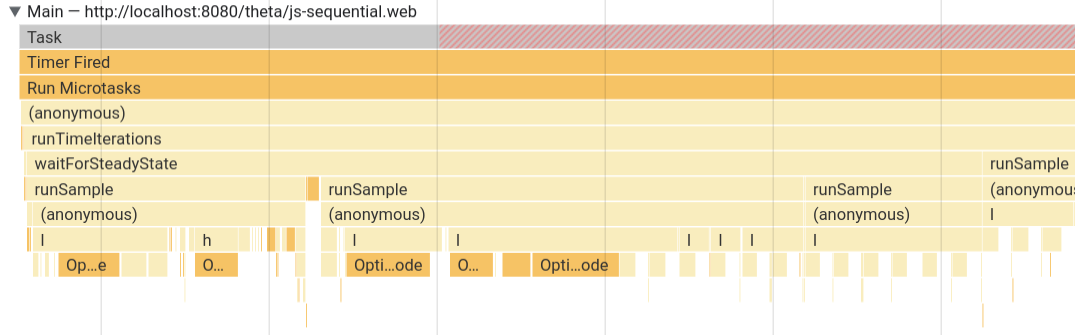
\includegraphics[width=\linewidth]{img/seq-profiler.png}
    \caption{Wynik profilowania wykonania sekwencyjnego algorytmu CHT w~przeglądarce Google Chrome.}
    \label{fig:profiler-seq}
\end{figure}

Zbadano również różnicę pomiędzy wartościami akumulatorów, która pomiędzy wariantami \textit{non-LUT} i~\textit{LUT} powinna być równa zero. Wykryto jednak różnicę dla jednego piksela, która widoczna jest na rysunku \ref{fig:diff:seq_lut}. Pochodzić ona może z~różnicy w~precyzji operacji zmiennoprzecinkowych. Tablica LUT funkcji trygonometrycznych zbudowana została z~wykorzystaniem pojedynczej precyzji i~obiektu tablicy typu \lstinline{Float32Array}. JavaScript wewnętrznie do reprezentacji liczb zmiennoprzecinkowych używa podwójnej precyzji.



\begin{figure}
    \groupBenchmark{
        \plotBenchmark{cpp_theta_SHT_Simple.csv}{cppColor}{{}}
        \addlegendentry{C++}

        \plotBenchmark{js-sequential_theta_SHT_Simple_node.csv}{nodeColor}{{}}
        \addlegendentry{Node}

        \plotBenchmark{js-sequential_theta_SHT_Simple_deno.csv}{denoColor}{{}}
        \addlegendentry{Deno}

        \plotBenchmark{js-sequential_theta_SHT_Simple_Firefox.csv}{firefoxColor}{{}}
        \addlegendentry{Firefox}

        \plotBenchmark{js-sequential_theta_SHT_Simple_Chrome.csv}{chromeColor}{{}}
        \addlegendentry{Chrome}

    } {
        \plotBenchmark{cpp_theta_SHT_Simple_Lookup.csv}{cppColor}{{}}
        \addlegendentry{C++}

        \plotBenchmark{js-sequential_theta_SHT_Simple_Lookup_node.csv}{nodeColor}{{}}
        \addlegendentry{Node}

        \plotBenchmark{js-sequential_theta_SHT_Simple_Lookup_deno.csv}{denoColor}{{}}
        \addlegendentry{Deno}

        \plotBenchmark{js-sequential_theta_SHT_Simple_Lookup_Firefox.csv}{firefoxColor}{{}}
        \addlegendentry{Firefox}

        \plotBenchmark{js-sequential_theta_SHT_Simple_Lookup_Chrome.csv}{chromeColor}{{}}
        \addlegendentry{Chrome}
    } {
        \plotBenchmark{cpp_theta_CHT_Simple.csv}{cppColor}{{}}
        \addlegendentry{C++}

        \plotBenchmark{js-sequential_theta_CHT_Simple_node.csv}{nodeColor}{{}}
        \addlegendentry{Node}

        \plotBenchmark{js-sequential_theta_CHT_Simple_deno.csv}{denoColor}{{}}
        \addlegendentry{Deno}

        \plotBenchmark{js-sequential_theta_CHT_Simple_Firefox.csv}{firefoxColor}{{}}
        \addlegendentry{Firefox}

        \plotBenchmark{js-sequential_theta_CHT_Simple_Chrome.csv}{chromeColor}{{}}
        \addlegendentry{Chrome}
    }
    [3400][850][14]
    \caption{Wyniki pomiarów czasu wydajności dla wykonania sekwencyjnego SHT i CHT.}
    \label{plot:sequential}
\end{figure}


\begin{figure}[h]
    \begin{subfigure}{0.3\textwidth}
        
\includegraphics[width=\linewidth] {../../packages/js-benchmarks/img/diff_seq_seq_lookup.png}
        \caption{SHT Sekwencyjny \textit{LUT}}\label{fig:diff:seq_lut}
    \end{subfigure}\hfill
    \begin{subfigure}{0.3\textwidth}
        
\includegraphics[width=\linewidth] {../../packages/js-benchmarks/img/diff_seq_wasm.png}
        \caption{SHT WASM}\label{fig:diff:wasm}
    \end{subfigure}\hfill
    \begin{subfigure}{0.3\textwidth}
        
\includegraphics[width=\linewidth] {../../packages/js-benchmarks/img/diff_seq_gpu.png}
        \caption{SHT WebGL}\label{fig:diff:gpu}
    \end{subfigure}
    \caption{Znormalizowana do przedziału $\lbrack 0, 255\rbrack$ absolutna różnica wartości akumulatorów z~wynikiem głosowania pomiędzy wykonaniem sekwencyjnym SHT \textit{non-LUT}.}\label{fig:diff}
\end{figure}



\section{NodeJS Native C++ Addon}

Implementacja natywnego modułu w~środowisko NodeJS wymaga utworzenia, oprócz właściwego kodu w~języku C++, warstwy abstrakcji, która zapewnia obsługę interfejsu po stronie języka JavaScript, pozwala na określenie typów zmiennych, kopiowanie danych, czy wywoływanie funkcji. Warstwa ta zaimplementowana została za pomocą Node-API, która dostarcza niezbędne interfejsy i~funkcje w~języku C++, aby efektywnie powiązać kod C++ i~JavaScript~\cite{napi}. Implementacja natywnych modułów korzysta dokładnie z~tego samego kodu, dla którego przeprowadzony pomiary w~natywnym C++. Kod ten został skompilowany do postaci bibliotek współdzielonych, które w~procesie linkowania jest dołączany do natywnego modułu NodeJS. 

Na listingu \ref{fig:nodejs} przedstawiony został plik z~paczki \textit{node-cpp-sequential}, który dołącza nagłówki z~paczki \textit{cpp-sequential}. Funkcja \lstinline{Napi::Object Init(Napi::Env env, Napi::Object exports)} zwraca obiekt, który definiuje wartości eksportowane przez moduł. W~niej właśnie definiowane są funkcje takie jak \lstinline{SHTSimple}, której implementację stanowi \lstinline{SHTSimpleBind}. Funkcja ta odpowiedzialna jest za stworzenie obiektów z~danymi wejściowymi zgodnie z~interfejsem dołączanych bibliotek (\lstinline{getTestImage} oraz \lstinline{getSHTOptions}), wywołania właściwej funkcji oraz zbudowanie obiektu z~odpowiedzią (\lstinline{getSHTResultBind}).

\begin{lstlisting}[language=C++, float=h, caption=Plik powiązania kodu C++ z~JavaScript, label=lst:cpp-js]
#define NAPI_DISABLE_CPP_EXCEPTIONS
#include "CHTSimple.h"
#include "SHTSimple.h"
#include "SHTSimpleLookup.h"
#include "napi.h"
#include <cstdint>

using namespace Napi;
    
Napi::Object SHTSimpleBind(const Napi::CallbackInfo &info) {
    Napi::Env env = info.Env();
    auto testImageBind = info[0].As<Napi::Uint8Array>();
    auto testImage = getTestImage(testImageBind);
    auto optionsBind = info[1].As<Napi::Object>();
    SHTOptions options = getSHTOptions(optionsBind);
    SHTResults results = SHTSimple(testImage, options);
  
    return getSHTResultBind(env, options, results);
  }
// ...
Napi::Object Init(Napi::Env env, Napi::Object exports) {
    exports.Set(Napi::String::New(env, "SHTSimple"),
                Napi::Function::New(env, SHTSimpleBind));
    // ...
    return exports;
}
  
NODE_API_MODULE(addon, Init)
\end{lstlisting}



\begin{figure}
    \groupBenchmark{
        \plotBenchmark{cpp-addon_theta_SHT_Simple_node.csv}{nodeColor}{{}}
        \addlegendentry{Node}

        \seqReference
    } {
        \plotBenchmark{cpp-addon_theta_SHT_Simple_Lookup_node.csv}{nodeColor}{{}}
        \addlegendentry{Node}

        \seqReferenceLookup
    }[1600][650]
    \label{plot:gpu}
    \caption{Node C++ addon SHT execution benchmark results.}
\end{figure}


\subsection{Wyniki pomiarów}

Na rysunku \ref{plot:cpu-addon} widać, że wykorzystanie tej metody akceleracji w~każdym przypadku przyspieszyło działania algorytmu względem odpowiadającego mu wykonania sekwencyjnego w~środowisku NodeJS. Przyspieszenie nastąpiło również względem wszystkich innych środowisk poza przypadkiem wariantu SHT \textit{LUT}, gdzie wydajność osiągnęła poziom wydajności odpowiednika wykonania sekwencyjnego w~przeglądarce Google Chrome.

Wariant SHT \textit{LUT} był \tms{4.40} szybszy od SHT \textit{non-LUT}, co wraz z~wynikami algorytmu CHT pozwala wyciągnąć wniosek, że jeśli w~algorytmie nie znamy z~góry niezbędnych wartości funkcji trygonometrycznych lub obliczenia są oparte głównie na liczbach całkowitych, to wykorzystanie tej metody akceleracji przynosi poprawę wydajności algorytmów. Oczywiście nie można zapominać o~wadach takiego rozwiązania, jaką stanowi konieczność implementacji warstwy wiążącej obydwa języki. Istnieje również konieczność zapewnienia kompatybilności biblioteki z~różnymi środowiskami uruchomieniowymi, dla których biblioteka musi zostać zbudowana zawczasu, lub w~momencie instalacji.

\section{WebAssembly i~asm.js}

Budowanie biblioteki wykorzystujące WebAssembly, tak jak w~przypadku natywnych modułów NodeJS, wymaga wykorzystania specyficznych narzędzi. Do budowy biblioteki we wszystkich wariantach wykorzystany został Emscripten \cite{emscripten} - zestaw narzędzi, dzięki którym dowolny przenośny kod w~językach kompatybilnych z~backendem kompilatora LLVM może został skompilowany do WebAssembly. Możliwym stało się uruchamianie w~środowiskach webowych kodu języków takich jak Python czy Lua, poprzez kompilację interpreterów tych języków.

\subsection{Implementacja procesu budowania}

Na listingu \ref{lst:wasm-build} przedstawiono wywołanie komendy \lstinline{emcc}, które inicjuje proces kompilacji. Z~perspektywy modularności oraz wygody użytkowania niezbędne jest omówienie opcji dostarczonych do komendy. Flaga \lstinline{--bind} uruchamia narzędzie Embind i~dodaje do kodu wynikowego modułu powiązania pomiędzy funkcjami eksportowanymi przez moduł, a~tymi zdefiniowanymi w~kodzie C++. Na listingu \ref{lst:wasm-bind} pokazano część kodu definiującego warstwę powiązania obydwu języków. Aby zapewnić zgodność z~docelowym interfejsem funkcja \lstinline{SHTSimpleBind} eksportowana jest jako \lstinline{SHTSimple}. W~porównaniu do natywnych modułów NodeJS w~tym wypadku Embind sam zajmuje się przetwarzaniem obiektów wejściowych na podstawie dostarczonych odwzorowań (linijka 16) i~powiązane funkcje zamiast argumentu z~całym kontekstem, otrzymać mogą argumenty w~docelowych typach. Jednak również tutaj wszystkie dane muszą zostać skopiowane do liniowego modelu pamięci WebAssembly. Za przetwarzanie obrazu wejściowego do postaci wektora liczb w~formacie \lstinline{uint8_t} odpowiedzialna jest funkcja \lstinline{emscripten::convertJSArrayToNumberVector}, która wymusza traktowanie wartości jako liczby, wpływając pozytywnie na wydajność. Opcja \lstinline{ALLOW_MEMORY_GROWTH=1} umożliwia powiększenie obszaru pamięci, który domyślnie ma rozmiar 16.0MB, co może nie wystarczyć, aby pomieścić przestrzeń akumulatora dla większych wartości próbkowania. Aby wynik kompilacji funkcjonował jako biblioteka eksportująca moduł ES6, należy użyć flag \lstinline{--no-entry} oraz opcji \lstinline{EXPORT_ES6=1}, \lstinline{MODULARIZE} oraz \lstinline{SINGLE_FILE=1}, aby binarny kod WebAssembly był zagnieżdżony w~pliku \lstinline{*.mjs} w~postaci kodu \textit{base64}. Nie można również zapomnieć o~możliwościach optymalizacji samego kompilatora, czyli o~flagach \lstinline{-O3}, czy \lstinline{-ffast-math}, która wprowadza optymalizacje działań matematycznych rezygnując z~poprawności wyników na ostatnich bitach.

\begin{lstlisting}[language=bash, float=ht, label=lst:wasm-build, caption=Komenda wykorzystana podczas kompilacji kodu C++ do modułu WebAssembly., showstringspaces=false]
COMMON_ARGS="-Inode_modules/cpp-sequential/include 
    --bind \
    -s MODULARIZE \
    -s ALLOW_MEMORY_GROWTH=1 \
    -s FILESYSTEM=0 \
    -s SINGLE_FILE=1 \
    -s ENVIRONMENT=web \
    -s EXPORT_ES6=1 \
    --no-entry \
    -std=c++17\
    -ffast-math\
    -O3"

### Non-SIMD
NON_SIMD_ARGS="$COMMON_ARGS \
    src/wasm_sequential.cc \
    node_modules/cpp-sequential/src/SHTSimpleLookup.cpp \
    node_modules/cpp-sequential/src/SHTSimple.cpp \
    node_modules/cpp-sequential/src/CHTSimple.cpp"

emcc $(echo $NON_SIMD_ARGS -o build/wasmSequential.mjs)
\end{lstlisting}

\begin{lstlisting}[language=C++, float=ht, label=lst:wasm-bind, caption=Wybrane fragmenty kodu warstwy powiązania WASM pomiędzy C++ i~JavaScript.]
// ...
#include <emscripten.h>
#include <emscripten/bind.h>

extern "C" {
// ...
EMSCRIPTEN_KEEPALIVE
SHTResults SHTSimpleBind(emscripten::val binaryImageBind, SHTOptions options) {
  auto testImage =
      emscripten::convertJSArrayToNumberVector<uint8_t>(binaryImageBind);
  return SHTSimple(testImage, options);
}
// ...
}

EMSCRIPTEN_BINDINGS(wasm_sequential) {
  emscripten::register_vector<uint32_t>("VectorUint32");
  emscripten::register_vector<uint8_t>("VectorUint8");
  emscripten::value_object<SHTSamplingOptions>("SHTSamplingOptions")
      .field("rho", &SHTSamplingOptions::rho)
      .field("theta", &SHTSamplingOptions::theta);
  // ...
  emscripten::function("SHTSimple", &SHTSimpleBind);
  // ...
}
\end{lstlisting}

\subsection{Warianty testów}

Dla każdego wariantu algorytmu transformacji przewidziano pomiary wydajności dla każdej z~wymienionych niżej metod.

\begin{itemize}
    \item asm.js -- wydajny podzbiór języka JavaScript zoptymalizowany pod kątem możliwości optymalizacji silnika i~inferencji typów,
    \item WASM -- standardowy wynik kompilacji kodu C++
    \item WASM SIMD (implicite) -- wynik kompilacji kodu C++ z~włączonym procesem automatycznej wektoryzacji wykonania, w~celu wykorzystania instrukcji wektorowych SIMD,
    \item WASM SIMD (explicite) -- wynik kompilacji kodu C++ z~ręcznie przeprowadzonym procesem wektoryzacji wykonania.
\end{itemize}

Zbudowanie biblioteki w~asm.js wymaga dodania opcji \lstinline{WASM=0}. Wariant SIMD explicite i~implicite budowany jest z~dodatkową flagą \lstinline{-msimd128}. Wariant SIMD explicite jest ręcznie przystosowany do obsługi operacji na wektorowych rejestrach 128b. Przykładem takiego zastosowania jest pokazana na listingu \ref{lst:simd} funkcja obliczająca minimalne i~maksymalne współrzędne w~przestrzeni akumulatora za jednym razem dla osi OX i~OY. W~procesie implementacji wersji SIMD explicite wykorzystano operacje na czteroelementowych wektorach liczb całkowitych bądź zmiennoprzecinkowych dla każdej intensywnie obliczeniowo pętli redukując liczbę ich iteracji czterokrotnie.

\begin{lstlisting}[language=C++, float=ht, label=lst:simd, caption=Funkcja \lstinline{getBounds} algorytmu CHT z~wykorzystaniem instrukcji SIMD.]
#include <wasm_simd128.h>
/ ...
void getBounds(int32_t x, int32_t max, v128_t vRBounds, int32_t *out) {
  v128_t vZero = wasm_i32x4_const_splat(0);
  v128_t vMax = wasm_i32x4_splat(max);
  v128_t vX = wasm_i32x4_splat(x);
  vX = wasm_i32x4_add(vRBounds, vX);
  vX = wasm_i32x4_max(vX, vZero);
  vX = wasm_i32x4_min(vX, vMax);
  wasm_v128_store(out, vX);
}
\end{lstlisting}



\begin{figure}[ht]
    \groupBenchmark{
        \plotBenchmark{js-asm_theta_SHT_Simple_node.csv}{nodeColor}{{}}
        \addlegendentry{Node}

        \plotBenchmark{js-asm_theta_SHT_Simple_Firefox.csv}{firefoxColor}{{}}
        \addlegendentry{Firefox}

        \plotBenchmark{js-asm_theta_SHT_Simple_Chrome.csv}{chromeColor}{{}}
        \addlegendentry{Chrome}

        \seqReference
    } {
        \plotBenchmark{js-asm_theta_SHT_Simple_Lookup_node.csv}{nodeColor}{{}}
        \addlegendentry{Node}

        \plotBenchmark{js-asm_theta_SHT_Simple_Lookup_Firefox.csv}{firefoxColor}{{}}
        \addlegendentry{Firefox}

        \plotBenchmark{js-asm_theta_SHT_Simple_Lookup_Chrome.csv}{chromeColor}{{}}
        \addlegendentry{Chrome}

        \seqReferenceLookup
    }{
        \plotBenchmark{js-asm_theta_CHT_Simple_node.csv}{nodeColor}{{}}
        \addlegendentry{Node}

        \plotBenchmark{js-asm_theta_CHT_Simple_Firefox.csv}{firefoxColor}{{}}
        \addlegendentry{Firefox}

        \plotBenchmark{js-asm_theta_CHT_Simple_Chrome.csv}{chromeColor}{{}}
        \addlegendentry{Chrome}

        \seqReferenceCircle
    }[9000][2300][25]
    \caption{Wyniki pomiarów czasu wydajności dla wykonania SHT i CHT z wykorzystaniem kompilacji do asm.js.}
    \label{plot:asm}
\end{figure}


\begin{figure}[h]
    \groupBenchmark{
        \plotBenchmark{js-wasm_theta_SHT_Simple_node.csv}{nodeColor}{{}}
        \addlegendentry{Node}

        \plotBenchmark{js-wasm_theta_SHT_Simple_Firefox.csv}{firefoxColor}{{}}
        \addlegendentry{Firefox}

        \plotBenchmark{js-wasm_theta_SHT_Simple_Chrome.csv}{chromeColor}{{}}
        \addlegendentry{Chrome}

        \seqReference
    } {
        \plotBenchmark{js-wasm_theta_SHT_Simple_Lookup_node.csv}{nodeColor}{{}}
        \addlegendentry{Node}

        \plotBenchmark{js-wasm_theta_SHT_Simple_Lookup_Firefox.csv}{firefoxColor}{{}}
        \addlegendentry{Firefox}

        \plotBenchmark{js-wasm_theta_SHT_Simple_Lookup_Chrome.csv}{chromeColor}{{}}
        \addlegendentry{Chrome}

        \seqReferenceLookup
    } {
        \plotBenchmark{js-wasm_theta_CHT_Simple_node.csv}{nodeColor}{{}}
        \addlegendentry{Node}

        \plotBenchmark{js-wasm_theta_CHT_Simple_Firefox.csv}{firefoxColor}{{}}
        \addlegendentry{Firefox}

        \plotBenchmark{js-wasm_theta_CHT_Simple_Chrome.csv}{chromeColor}{{}}
        \addlegendentry{Chrome}

        \seqReferenceCircle
    }[2500][950][15]
    \caption{Wyniki pomiarów czasu wydajności dla wykonania SHT i CHT z wykorzystaniem kompilacji do WASM.}
    \label{plot:wasm}
\end{figure}


\begin{figure}[h]
    \groupBenchmark{
        \plotBenchmark{js-wasm_simd_explicit_theta_SHT_Simple_node.csv}{nodeColor}{{}}
        \addlegendentry{Node}

        \plotBenchmark{js-wasm_simd_explicit_theta_SHT_Simple_Firefox.csv}{firefoxColor}{{}}
        \addlegendentry{Firefox}

        \plotBenchmark{js-wasm_simd_explicit_theta_SHT_Simple_Chrome.csv}{chromeColor}{{}}
        \addlegendentry{Chrome}

        \seqReference
    } {
        \plotBenchmark{js-wasm_simd_explicit_theta_SHT_Simple_Lookup_node.csv}{nodeColor}{{}}
        \addlegendentry{Node}

        \plotBenchmark{js-wasm_simd_explicit_theta_SHT_Simple_Lookup_Firefox.csv}{firefoxColor}{{}}
        \addlegendentry{Firefox}

        \plotBenchmark{js-wasm_simd_explicit_theta_SHT_Simple_Lookup_Chrome.csv}{chromeColor}{{}}
        \addlegendentry{Chrome}

        \seqReferenceLookup
    }{
        \plotBenchmark{js-wasm_simd_explicit_theta_CHT_Simple_node.csv}{nodeColor}{{}}
        \addlegendentry{Node}

        \plotBenchmark{js-wasm_simd_explicit_theta_CHT_Simple_Firefox.csv}{firefoxColor}{{}}
        \addlegendentry{Firefox}

        \plotBenchmark{js-wasm_simd_explicit_theta_CHT_Simple_Chrome.csv}{chromeColor}{{}}
        \addlegendentry{Chrome}

        \seqReferenceCircle
    }[2200][650][15]
    \caption{Wyniki pomiarów czasu wydajności dla wykonania SHT i CHT z wykorzystaniem kompilacji do WASM z ręczną implementacją instrukcji SIMD.}
    \label{plot:wasm_simd_explicit}
\end{figure}



\subsection{Wyniki pomiarów}

Analizując wykres przedstawiający wyniki pomiarów czasów wykonania algorytmów z~wykorzystaniem kompilacji do asm.js przedstawiony na rysunku \ref{plot:asm} zobaczyć można, że ta metoda akceleracji w~każdym przypadku daje gorsze rezultaty od wykonania sekwencyjnego. Może to mieć dwie potencjalne przyczyny. Pierwszą z~nich jest nieprzeprowadzanie kompilacji kodu przez środowiska, które z~asm.js nie są w~pełni kompatybilne, co w~przypadku tych konkretnych algorytmów powoduje utratę wydajności. W~zbudowanym module nie znajdują się funkcje trygonometryczne \lstinline{Math.sin} i~\lstinline{Math.cos}. Oznacza to, że w~kodzie znajduje się ich ręczna implementacja, która nie korzysta z~biblioteki standardowej. Drugim możliwym powodem, w~szczególności w~przypadku przeglądarki Mozilla Firefox, która z~asm.js jest w~pełni kompatybilna, może być problem z~wykrywaniem kodu asm.js, który jest umieszczony w~jednej paczce z~resztą kodu w~procesie budowania. Świadczyć może o~tym fakt, że podczas profilowania wykonania nie występowały bloki \textit{Compile}, co ma miejsce podczas wykonania wyizolowanych przykładów.

Kompilacja do WebAssembly zwiększyła wydajność wariantu algorytmu SHT \textit{non-LUT} we wszystkich testowanych środowiskach (rys. \ref{plot:wasm}). Jednak największy wpływ miała na środowiska przeglądarek internetowych, które zdają się lepiej reagować na te metodę akceleracji niż środowisko NodeJS. W~wariancie SHT \textit{LUT} za to nie zaobserwowano żadnej poprawy względem wykonania sekwencyjnego. dodatkowo nie zaobserwowano optymalizacji czasu wykonania dla $S_\theta \geq 5$. Warianty te różnią się jedynie zmniejszoną liczbą wywołać funkcji trygonometrycznych. Założyć można zatem, że zaobserwowana optymalizacja przeglądarki Mozilla Firefox dotyczyła właśnie ich i~nie odbyła w~momencie kompilacji do WebAssembly. 

Przypadek algorytmu CHT pokazuje jak różne środowiska mogą reagować na ten sam kod. W~przeglądarce Google Chrome z~silnikiem V8 zaobserwowano poprawę wydajności, gdzie wykonanie z~wykorzystaniem WebAssembly było \tms{1.70} szybsze od wykonania sekwencyjnego dla $n = 1$. Mozilla Firefox jednak zachowuje się inaczej. Dla $n = 1$ wykonanie z~wykorzystaniem WebAssembly było \tms{1.63} szybsze, niż wykonanie sekwencyjne, jednak dla $n = 10$ czas wykonania był już taki sam jak czas wykonania sekwencyjnego. Na tej podstawie można wyciągnąć wniosek, że w~przypadku przeglądarki Mozilla Firefox duża liczba iteracji generuje narzut, który niweluje korzyści, jakie płyną z~ogólnej poprawny wydajności dzięki WebAssembly. 

Kompilacja do WebAssembly z~włączonym procesem automatycznej wektoryzacji w~narzędziu Emscripten nie przyniosła żadnej różnicy w~porównaniu do wykonania zwykłego kodu WebAssembly. Natomiast w~przypadku ręcznej optymalizacji, czego przykład pokazany został na listingu \ref{lst:simd}, poprawa wydajności zależała od środowiska. Na rysunku \ref{plot:wasm_simd_explicit} zaobserwować można, że wszystkie środowiska pozytywnie zareagowały na zastosowaną metodę dla wariantu algorytmu SHT \textit{non-LUT}. Najszybsza znów okazała się przeglądarka Google Chrome, osiągając wynik \tms{1.50} lepszy od wykonania sekwencyjnego. W~wariancie SHT \textit{LUT} jednak wykonanie sekwencyjne było \tms{1.15} szybsze. Wykonanie wariantu CHT w~przeglądarka Mozilla Firefox, w~porównaniu do wykonania sekwencyjnego, było wolniejsza, a~wykonanie w~środowiskach Google Chrome i~NodeJS zyskało na wydajności.

Dla analizowanego kąta obrotu $\theta = \frac{\pi}{2}$ wykryto duże różnice w~akumulatorze pomiędzy wykonaniem SHT WASM a~sekwencyjnym SHT. Różnica widoczna jest na rysunku \ref{fig:diff:wasm}. Oprócz wyraźnej linii różnica występuje też dla wielu pojedynczych pól akumulatora i~występować może z~różnicy w~reprezentacji w~algorytmie liczb zmiennoprzecinkowych, co generuje różnice w~wyliczeniach pól akumulatora.

\section{Współbieżność}

Zrównoleglenie wykonania bezdyskusyjnie przynosi wzrost wydajności. Jednak, aby mogło być zastosowane algorytm musi dać się zrównoleglić. Również docelowe środowiska muszą tę współbieżność wspierać. Wspólnym mianownikiem wszystkich badanych środowisk jest wielowątkowość w~postaci Worker'ów. Oprócz nich środowisko NodeJS posiada natywne mechanizmy komunikacji między procesami, jednak nie są one przedmiotem badań w~tej pracy.

Komunikacja pomiędzy Worker'ami odbywa się z~wykorzystaniem interfejsów WebWorker API. Dostarczają one mechanizm wiadomości, które są asynchronicznie przetwarzane przez Worker'y, które jako niezależne wątki mają osobną pętlę zdarzeń. Wiadomość jest w~abstrakcji przetwarzania zdarzeniem. Metoda \lstinline{Worker.postMessage(...)} oraz definiowana funkcja \lstinline{self.onmessage} pozwala na wysyłanie i~obsługę zdarzeń wiadomości pomiędzy wątkami. Mechanizm ten jest bardzo prosty, niweluje problemy wyścigów oraz współdzielenia zasobów, ponieważ wszystkie dane są albo kopiowane, albo transferowane z~jednego wątku do drugiego. Jego wadą jest sam interface, który wymaga tworzenia dodatkowych mechanizmów serializacji i~parsowania złożonych wiadomości. Z~pomocą przychodzi, zastosowana przy implementacji Worker'ów na potrzeby badan, biblioteka Comlink \cite{comlink}. Pozwala ona na zdalne wywoływanie funkcji i~synchronizację zmiennych, która interfejsem nie odbiega od sposobu interakcji z~metodami i~atrybutami obiektów. Jest ona kompatybilna ze wszystkimi badanymi środowiskami. 

Implementacja Worker'ów wymagała przystosowania algorytmów. Podzielono wykonanie głównych ich pętli pomiędzy wątki. W~testach badano czasy wykonania dla liczby wątków $c=4$. Aby zapewnić kompatybilność ze wszystkimi środowiskami konieczne było zbudowanie dwóch wersji biblioteki. Biblioteka w~środowisku Deno była uruchamiana z~pominięciem procesu budowania, ponieważ Deno pozwala bezpośrednio na uruchomienie kodu w~języku TypeScript. 

Dla środowiska przeglądarki internetowej konieczne jest użycie loader'a \lstinline{worker-loader}, który, z~opcją \lstinline{inline: 'no-fallback'}, odpowiedzialny jest za dołączenie kodu Worker'a do kodu biblioteki, aby taka biblioteka mogła być ponownie zbudowana razem z~docelową aplikacją. W~standardowym scenariuszu, kiedy Worker budowany jest razem z~aplikacją, Worker jest pobierany jako osobny plik przez przeglądarkę. Kod musi być dołączony w~tym samym pliku, ponieważ niemożliwym jest, bez dodatkowych skryptów, wskazanie i~skopiowanie pliku Worker'a w~procesie budowania.

Dla środowiska NodeJS konieczne jest jawne wskazanie środowiska, dla którego przeznaczona jest budowana biblioteka poprzez ustawienie opcji \lstinline{target: 'node'}. NodeJS do obsługi Worker'ów używa wbudowanego modułu, WebWorker API jest lekko zmodyfikowane, a~konstruktor obiektu \lstinline{Worker} nie jest dostępny jako symbol globalny. Narzędzie Webpack musi uwzględnić wszystkie te elementy. Niekompatybilność ta uniemożliwia w~wypadku tej metody akceleracji zbudowanie pliku kompatybilnego ze wszystkimi środowiskami. Na rysunku \ref{fig:workers-struct} przedstawiono diagram zależności modułów w~kodzie, w~tym adapterów, które zapewnia kompatybilność kodu algorytmu ze wszystkimi środowiskami. Kod części właściwego algorytmu, który tworzy i~wywołuje funkcje Worker'ów w~środowiska Deno jest oderwana od jego odpowiednika wspólnego dla przeglądarek i~NodeJS. Jest to spowodowane niekompatybilnością API biblioteki Comlink w~wersji na środowisko Deno.

\begin{figure}[h]
    \centering
    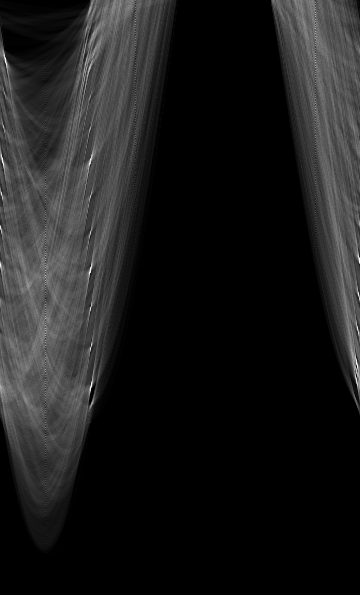
\includegraphics[width=\linewidth]{diagrams/out/workers.png}
    \caption{Sieć zależności pomiędzy modułami implementującymi algorytm SHT w~wersji \textit{non-LUT}, która zapewnia kompatybilność ze wszystkimi środowiskami.}
    \label{fig:workers-struct}
\end{figure}

\subsection{Wyniki pomiarów}

Pomiary dla wykonania wielowątkowego przeprowadzone były przy przeznaczonych do tego 4 fizycznych rdzeni procesora, aby uniknąć wpływu hyper-threading'u na czas wykonania. Wymagało to przypisania 8 wirtualnych rdzeni używając maski \lstinline{0x000000ff} jako konfiguracji narzędzia \lstinline{taskset}.



\begin{figure}
    \groupBenchmark{
        \plotBenchmark{js-workers_theta_SHT_Simple_node.csv}{nodeColor}{{}}
        \addlegendentry{Node}

        \plotBenchmark{js-workers_theta_SHT_Simple_deno.csv}{denoColor}{{}}
        \addlegendentry{Deno}

        \plotBenchmark{js-workers_theta_SHT_Simple_Firefox.csv}{firefoxColor}{{}}
        \addlegendentry{Firefox}

        \plotBenchmark{js-workers_theta_SHT_Simple_Chrome.csv}{chromeColor}{{}}
        \addlegendentry{Chrome}

        \seqReference
    } {
        \plotBenchmark{js-workers_theta_SHT_Simple_Lookup_node.csv}{nodeColor}{{}}
        \addlegendentry{Node}

        \plotBenchmark{js-workers_theta_SHT_Simple_Lookup_deno.csv}{denoColor}{{}}
        \addlegendentry{Deno}

        \plotBenchmark{js-workers_theta_SHT_Simple_Lookup_Firefox.csv}{firefoxColor}{{}}
        \addlegendentry{Firefox}

        \plotBenchmark{js-workers_theta_SHT_Simple_Lookup_Chrome.csv}{chromeColor}{{}}
        \addlegendentry{Chrome}

        \seqReferenceLookup
    }[1700][500]
    \label{plot:workers}
    \caption{Workers SHT execution benchmark results with concurrency $n=4$. Gray area shows sequential JavaScript execution performance range. Non-LUT variant performs better than sequential execution. On the other hand the LUT one has gained only small increase in performance.}
    % TODO: speedup math
\end{figure}


\begin{wraptable}{r}{6cm}
    \caption{Speedup metrics for worker acceleration method ($S_\theta = 1, p = 4$).}
    \label{tab:worker_speedup}
    \setlength{\tabcolsep}{0.5em}
    \begin{tabular}{lrr}%
        \hline
        Env.        & Speedup & Efficiency              \\
        \hline
        Chrome      & 2.99    & 0.75                    \\
        Firefox     & 2.82    & 0.70                    \\
        Node        & 3.25    & \textcolor{green!70!black}{0.81} \\
        Deno        & 2.70    & \textcolor{red}{0.67}   \\
        Chrome \textit{LUT}  & 1.85    & 0.46                    \\
        Firefox \textit{LUT} & 1.89    & 0.47                    \\
        Node \textit{LUT}    & 1.76    & 0.44                    \\
        Deno \textit{LUT}    & 1.51    & \textcolor{red}{0.38}   \\
        \hline
    \end{tabular}
\end{wraptable}

Na rysunku \ref{plot:workers} pokazane zostały wykresy z~wynikami pomiarów czasów wykonania z~wykorzystaniem czterech Worker'ów. Jak w~większości przypadków również i~tutaj, dla obydwu wariantów SHT, prym we wzroście wydajności wiedzie przeglądarka Google Chrome. Przy krótszych czasach wykonania dla wariantu CHT uwydatnia się większa niż dla poprzednich metod wartość odchylenia standardowego. Szczególnie widoczna jest w~przypadku przeglądarki Mozilla Firefox. Spowodowane jest to asynchronicznością komunikacji z~Worker'em, gdzie wiadomości nie są obsługiwane od razu, a~trafiają do pętli zdarzeń. W~zależności od implementacji, jak i~liczby zdarzeń do obsłużenia przez pętlę, czasy te mogą się różnić. Kod Worker'ów jest również osobno optymalizowany, co zwiększa skalę zjawiska zimnego startu w~przypadku tej metody akceleracji.  Na rysunku \ref{fig:profiler-workers} widać wynik profilowania pierwszych wykonań kody na stworzonych instancjach Worker'ów. W~pierwszych wykonaniach widać bloki \textit{Optimise Code}, a~dalsze wykonania wykonują się już po optymalizacji. Podczas długiej przerwy pomiędzy wykonaniami proces optymalizacji zachodził dla wątku głównego.

\begin{figure}[h]
    \centering
    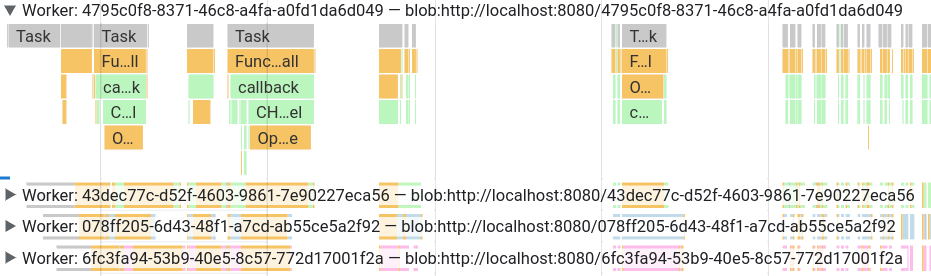
\includegraphics[width=\linewidth]{img/workers-profiler.png}
    \caption{Wynik profilowania wykonania algorytmu CHT w~przeglądarce Google Chrome z~użyciem Worker'ów.}
    \label{fig:profiler-workers}
\end{figure}

W tabeli \ref{tab:speedup} przedstawiono miarę przyspieszenia obliczeń oraz jej efektywność. Największe przyspieszenie, a~zarazem jego efektywność ma miejsce w~przypadku wariantu SHT \textit{non-LUT} i~środowiska NodeJS. Różnica wyników pomiędzy wariantami SHT \textit{non-LUT} i~SHT \textit{LUT} jest znacząca i~kolejny raz wskazuje na funkcje trygonometryczne i~ogólnie zmiennoprzecinkowe jako czynnik, na który trzeba zwrócić uwagę podczas optymalizacji algorytmów. W~wariancie CHT przyspieszenie jest niewielkie, ponieważ zrównolegleniu poddany został sam proces głosowania na środek okręgu. Jeśli w~danych wejściowych większa liczba pikseli byłaby zapalona, etap głosowania byłby bardziej wymagający, co zwiększyłoby efektywność przyspieszenia.

Worker'y współdzielą pamięć akumulatora w~postaci obiektu \lstinline{SharedArrayBuffer}. Z~uwagi na to, że każdy Worker działał na własnym fragmencie pamięci podczas procesu głosowania, nie było konieczne stosowanie operacji atomowych z~wykorzystaniem metod interfejsu \lstinline{Atomic}. Użycie takiego interfejsu spowalniało wykonanie algorytmu w~testach podczas implementacji. 


\section{GPGPU}

\subsection{Wyniki pomiarów}

